Friction is a difficult concept in elementary physics because it is the first type of non-conservative force that is often taught. The definition of a non-conservative force can be given by using multivariate calculus, or through a relatively simple physical explanation. If you have seen multivariate calculus, then a non-conservative force is a force that has a curl of 0. However, I assume most have not seen this, so, in a physical sense, a non-conservative force is a force that will do non-zero work if you move an object on a closed path(a loop). We will explore this topic furthermore when we talk about work, but for now, we think of friction as something that acts against the motion of an object regardless of whether the object is moving forward or backward. The reason why friction is not conservative we will not discuss technically. However, I think it is important you understand that friction, like the normal force, is the result of intermolecular forces at the layer between the two surfaces. Another important thing to understand is that the frictional force on an object is not constant. The frictional force on an object will increase until it reaches a certain peak amount which it stays at, or it may decrease from if enough force is applied to overcome the frictional force and cause the object to begin moving. For right now, we will discuss the frictional force when the object is not moving. This is called the static frictional force. To help us imagine the static force, I want you to imagine a block on a surface that is being pulled by force in one direction(F) and friction is working against the force. What must the value of the frictional force be? Well, if the acceleration of the body is 0(as it is at rest). Then  \begin{equation}F_{net}\left(x\right)=ma=0=F-F_{friction}\end{equation} The frictional force must take on the value of the force being applied to the object. And then, say that we all of a sudden drop the force by a certain amount. What happens? Well, physically, nothing should happen, the body should stay at rest. Friction can not cause the body to move in the direction of the frictional force. That would not make any sense. No, the body stays at rest and $F_{friction}$ lowers to the new force being applied to the body. So, when a body is at rest, the force of Friction is equal in magnitude to the force being applied to the body, but opposite in the other direction. So what happens as the force being applied to the body increases? Well, the frictional force can’t keep increasing forever, and it doesn’t. It increases up to a certain point after which any added force will cause the body to move. 

Kinetic friction is the friction that occurs when a body is moving.  Kinetic friction is perhaps easier to understand than static friction because, for our purposes, we can assume kinetic friction is not changing if we have a force being applied that is parallel to the frictional force. We saw kinetic friction when we did the example with the block moving down the ramp. The effect of friction was in the opposite direction of the force causing the motion and was perpendicular to the normal force.

Now that we understand the types of friction we can begin to discuss the value of the frictional force for dynamics problems. First, a fact is that the frictional force will vary linearly with the normal force. I like to think about this as making sense. Imagine we have a plane and a block moving across the plane. If we give the block a mass m, there will be a certain frictional force as the body moves. However, if we were to increase the mass of the block, it would at a molecular level at least “sink in” to the table a bit more due to the gravitational force, forcing the normal force to increase to prevent this. When the block sinks into the table a bit more, there is a larger frictional force as for the block to move at a molecular level; it has to descend into the table. This is certainly not an exact description of what is going on here, but it is a way to rationalize why friction would increase when we have a larger mass(and therefore a larger normal force). In practice, you can ignore this description and think of friction as being caused by inter-molecular bumps that require more energy to overcome the more the surfaces in contact are pushing on each other. 

Now we can attempt to do an example with the frictional force. Imagine that we have a plane on which an object is moving as seen below. 
\newline
\newline
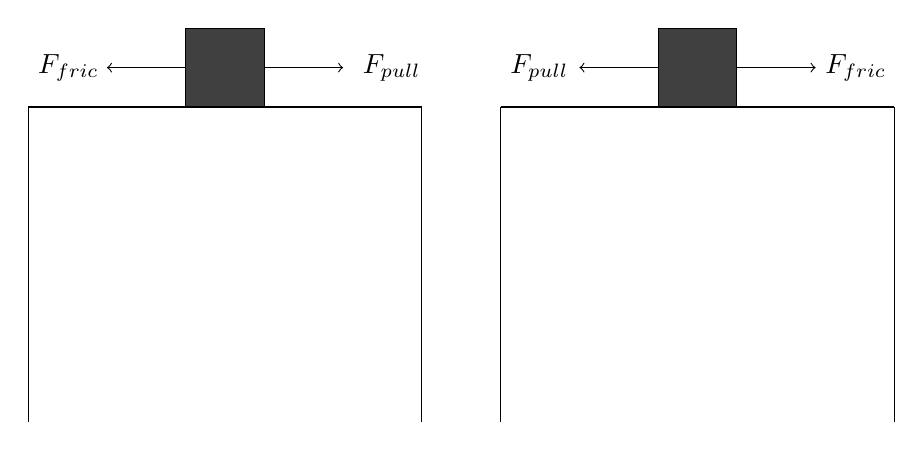
\begin{tikzpicture}
\filldraw[fill = darkgray, draw = black] (2,4) rectangle (3,5);
\filldraw[fill = darkgray, draw = black] (8,4) rectangle (9,5);
\filldraw[fill = darkgray, draw = black] (8,4) rectangle (9,5);
\draw[->] (3,4.5) -- (4,4.5);
\draw[->] (9,4.5) -- (10,4.5);
\draw[->] (2,4.5) -- (1,4.5);
\draw[->] (8,4.5) -- (7,4.5);
\draw[black] (4.125,4.5) node[anchor=west] {$F_{pull}$};
\draw[black] (0,4.5) node[anchor=west] {$F_{fric}$};
\draw[black] (6,4.5) node[anchor=west] {$F_{pull}$};
\draw[black] (10,4.5) node[anchor=west] {$F_{fric}$};
\draw[black] (0,0) -- (0,4);
\draw[black] (0,4) -- (5,4);
\draw[black] (5,4) -- (5,0);
\draw[black] (6,0) -- (6,4);
\draw[black] (6,4) -- (11,4);
\draw[black] (11,4) -- (11,0);
\end{tikzpicture}
\newline
A person is pulling it across the plane and a crane pulling the object up. We can assume that the object is only moving along the plane and not upwards. So we have a classic dynamics problem. We can use Newton’s laws in the x and y directions to create equations of motion that we can use here to find out how fast the object moves given the mass of the object. We are given $\vec{F_{Person}}$, $\mu_{kinetic}$, and $\vec{F_{Crane}}$. Here $\mu_{kinetic}$ is the coefficient of friction for a moving object, that is $\mu_{kinetic}\cdot F_{normal} = F_{friction}$ Once you have the equations given by Newton's law you have to use a certain physical insight to be able to solve the problem. So we have that \begin{equation}F_x=F_{person}-F_{friction}=ma_x\end{equation} and that \begin{equation}F_y=F_{crane}+F_{normal}-F_{Gravity}=ma_y\end{equation} However we know that $a_y=0$, $F_{gravity}=mg$, and that \begin{equation}F_{friction} =\mu F_{normal}\end{equation} So we can write that \begin{equation}0=F_{crane}+F_{normal}-mg\end{equation} And that \begin{equation}ma=F_{person}-\mu F_{normal}\end{equation} From these equations, we see that we know everything we need to find the acceleration other than the normal force. We can use the Eq. 3.4.2. to find the normal force through some simple algebra. We rearrange to find that $F_{normal}= mg-F_{crane}$. Plugging this into the Eq. 3.4.6, we get that \begin{equation}ma=F_{person}-\mu\left(mg-F_{crane}\right)\end{equation} and then we get that \begin{equation}a = \frac{F_{person}+F_{crane}}{m}-\mu g\end{equation} This is very interesting, and we should see if it makes physical sense. First, we see that if $\mu$ were to increase, then the acceleration would decrease. This makes sense because if $\mu$ were to increase, there would be a larger frictional force slowing down the object. We also see that if the mass of the object were to increase we would have a lower acceleration. This makes sense following the law of inertia. We also see that if $F_{person}$ were to increase, then the acceleration of the body would increase. This should also make sense. If there is a larger force pulling on the object trying to move it, then naturally we would have a larger acceleration. Lastly, if the force of the crane were to increase, then we would have a larger acceleration as well. We can rationalize this by looking at the equations which give us some physical insight into why this is. With the equations, we see that if the Force of the crane increases then the normal force decreases and therefore the frictional force decreases, causing a small frictional force. This is quite interesting, even though the crane is not even acting in the same direction as the motion of the object, it can still change its acceleration. 
